\subsubsection{Gabinete}

Una vez fabricadas y armadas las placas, se avanzó con el diseño de un gabinete para finalizar el diseño de hardware del prototipo. Considerando las medidas de las placas y que una de ellas funciona como parte del panel frontal del SAL/T, se realizó un diseño pensado para su fabricación en impresión 3D con medidas de 300 x 300 x 100mm. El panel frontal cuenta con los agujeros y espacios necesarios para que los LEDs, display y botones de la placa secundaria sean visibles por fuera. En la figura \ref{fig:gabinete_3d} se visualiza el diseño del gabinete.   

\begin{figure}[H]
    \centering
    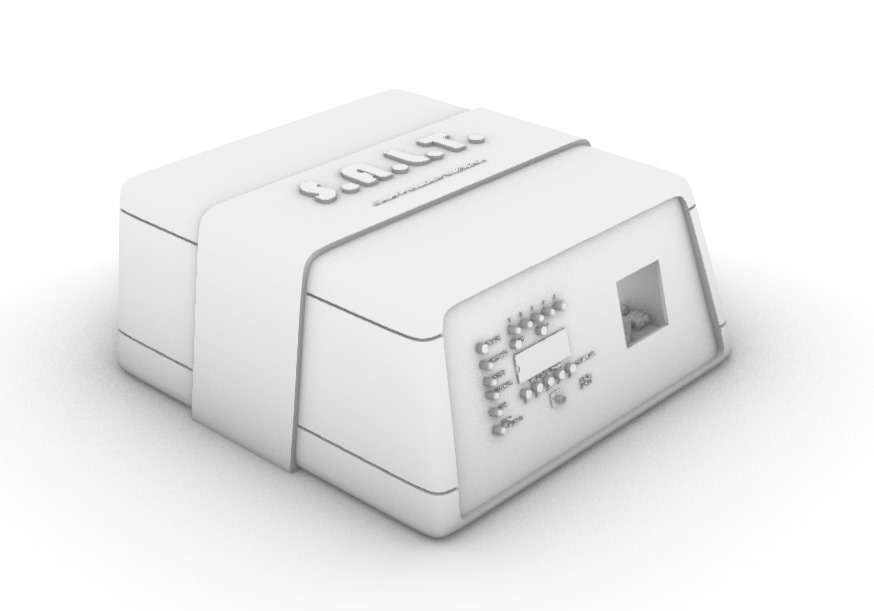
\includegraphics[width = \linewidth]{img/gabinete.jpeg}
    \caption{Diseño de gabinete para impresión 3D}
    \label{fig:gabinete_3d}
\end{figure}    

La fabricación del gabinete estaba pensada para realizarse utilizando la impresora 3D Prusa P3 Steel que tiene el Laboratorio Abierto (LABi) de la Facultad de Ingeniería de la Universidad de Buenos Aires \cite{labi_3d}. Considerando las dimensiones máximas que se pueden fabricar por pieza, se realizó la división del prototipo en 22 piezas que no excedan las dimensiones de 19 x 19cm. \\ 

Una vez finalizada la separación de las partes, se realizó la consulta con el LABi para su fabricación y, si bien el diseño y las piezas eran fabricables de manera individual, la fabricación del prototipo entero requería de demasiadas horas de uso de la impresora y demasiado material plástico debido a su gran tamaño y a la velocidad de fabricación del modelo de la impresora, lo que implicaba un costo innecesariamente alto para la fabricación del prototipo. \\ 

Por lo tanto, se siguieron las recomendaciones de utilizar un gabinete prefabricado para contener las placas del prototipo y realizar los ajustes necesarios para conseguir un panel frontal indicativo similar al diseñado previamente. Los gabinetes pensados para placas electrónicas son de menor dimensión, por lo que no se pudo conseguir ninguna para el prototipo. Finalmente, se consiguió un gabinete pensado para instalaciones eléctricas de 310 x 310 x 110mm con tapa atornillable que resultó ideal para el prototipo; el modelo es una caja estanca plástica blanca IP65 de Sistelectric, una empresa de Genrod \cite{gabinete}. El gabinete conseguido con las modificaciones realizadas se puede visualizar en la figura \ref{fig:gabinete_fabricado}. Las placas están atornilladas al gabinete y montadas sobre unos pequeños separadores para permitir que la placa no queda apoyada ni en contacto con el gabinete. 

\begin{figure}[H]
    \centering
    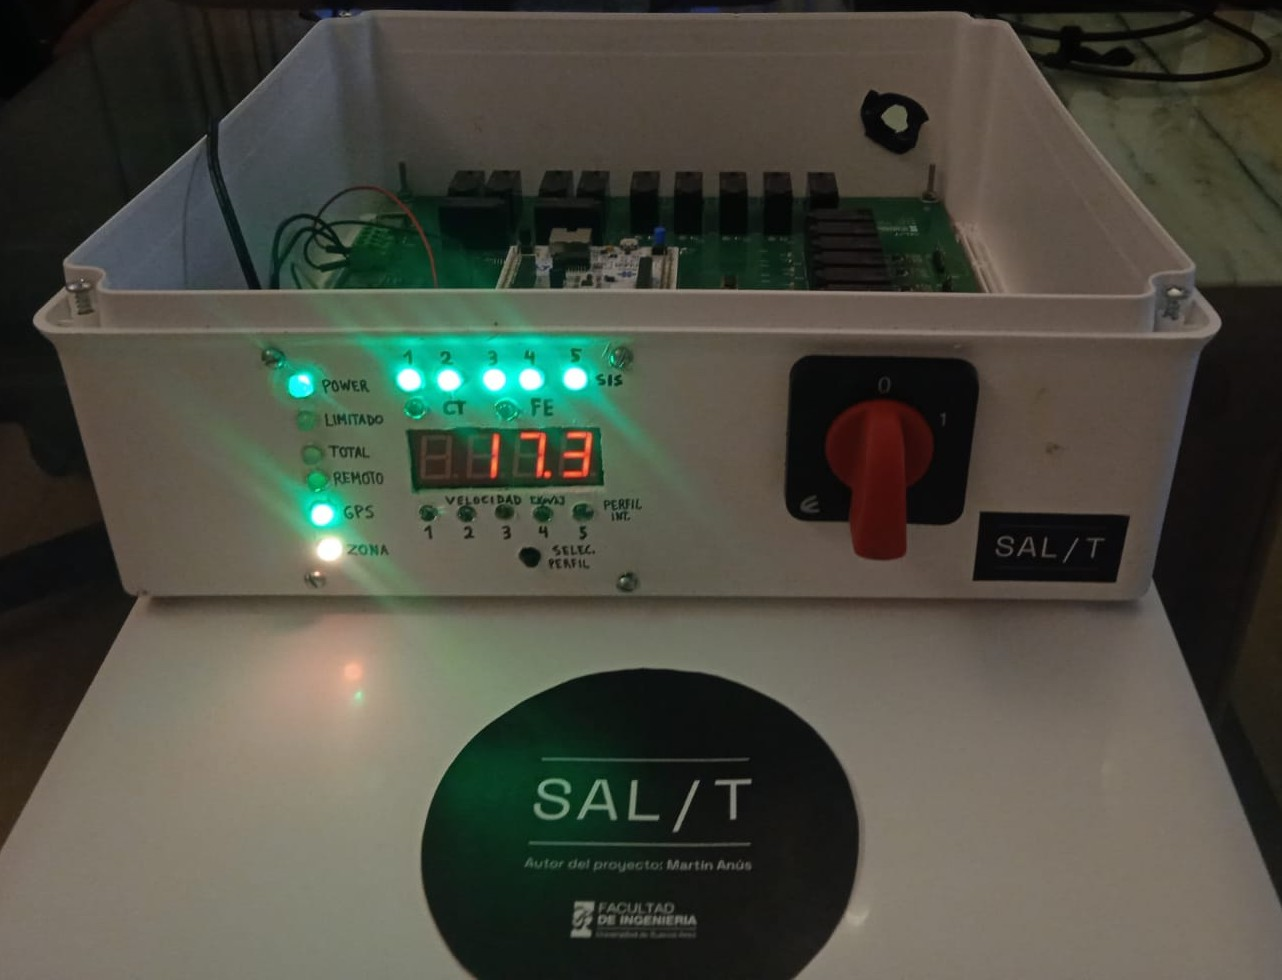
\includegraphics[width = \linewidth]{img/salt_fabricado.jpeg}
    \caption{Gabinete acondicionado para el prototipo del SAL/T}
    \label{fig:gabinete_fabricado}
\end{figure} 

Se realizaron las perforaciones necesarias para el panel frontal y la llave de activación. En la figura \ref{fig:frente_fabricado} se visualiza el frente del gabinete con la placa insertada y la llave de activación del modo aislado total. 

\begin{figure}[H]
    \centering
    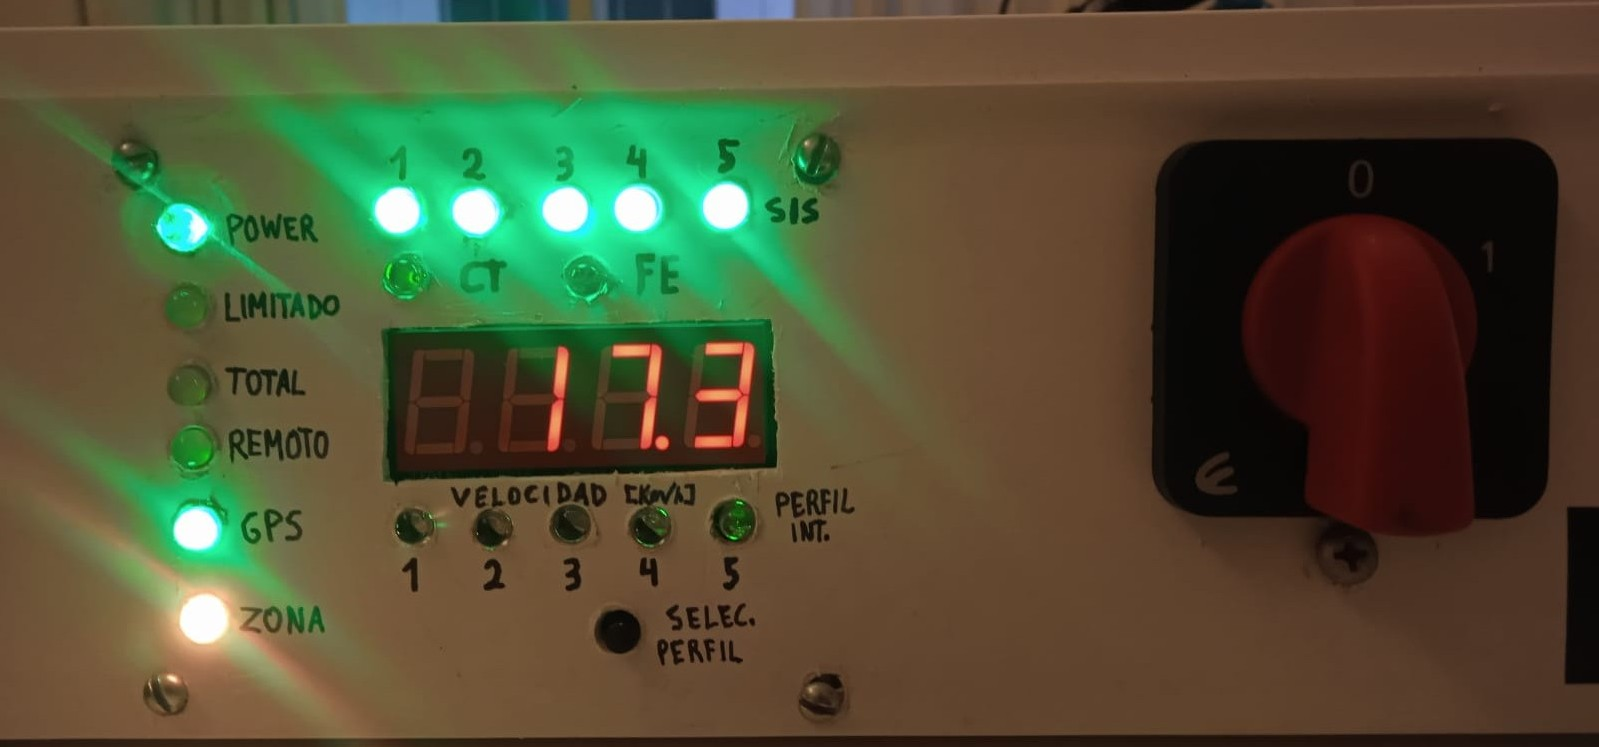
\includegraphics[width = \linewidth]{img/frente_fabricado.jpeg}
    \caption{Frente del del prototipo del SAL/T}
    \label{fig:frente_fabricado}
\end{figure} 